\documentclass{beamer}
\usepackage{amsmath, amsfonts, amssymb, amsthm}
\usepackage{graphicx, caption, hyperref, url, cite}
\usepackage[UTF8, noindent]{ctexcap}
\usepackage{listings}

\usetheme{Boadilla}

\title{汇报0608}
% \subtitle{项目三:基于大规模预训练模型的生成式知识问答}
\institute{项目三}
\author{朱睿涵 \and 李宸亦}
\date{\today}

\setbeamertemplate{bibliography item}[text]

\begin{document}

\frame{\titlepage} % 标题页

\AtBeginSection{
    \begin{frame}
        \frametitle{目录}

        \tableofcontents[currentsection]
    \end{frame}
}


\section{抽取式阅读理解}

\begin{frame}
    \frametitle{上周工作}

    \begin{enumerate}
        \item 将模型中单一score指标增加到AVERAGE,F1 score和EM。主要根据F1score进行评估
        % \tiny "AVERAGE": "10.601", "F1": "17.878", "EM": "3.324"
        \item 尝试将观点类问题和no answer问题加入模型中,但是效果较差。
    \end{enumerate}

    \begin{figure}
        \centering
        
\includegraphics[width=0.8\textwidth]{fig/pic1.png}
    \end{figure}

    \begin{figure}
        \centering
        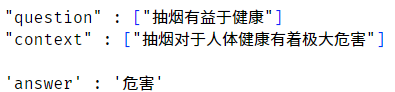
\includegraphics[width=0.5\textwidth]{fig/pic.png}
    \end{figure}


\end{frame}



\begin{frame}
    \frametitle{预计工作}

    \begin{itemize}
        \item 确保基础事实性阅读理解的效果,并进行封装,将主要注意力集中在封装API上。
        \item 继续尝试提高观点类问题回答的效果。
    \end{itemize}

\end{frame}

\section{生成式阅读理解}
\subsection{问题}
\begin{frame}[fragile]{问题}
    在实际运行新的多任务模型时发现效果非常差(F1仅为0.07左右)

    暂时没有确定出现bug的原因,目前猜测的问题:

    \begin{itemize}
        \item loss:目前用的是 $L = \alpha L_g + (1 - \alpha)L_c$ 的总loss,$\alpha = 0.5$,有可能这两个损失函数减小的速度差距悬殊,答案生成主任务反而被完全掩盖了。
        \item eval:计算F1 score的时候只评判预测answer和测试集answer,实际上并没有将yes no观点纳入考虑。
        \item 问题分类任务是否真的对答案生成任务有帮助?
    \end{itemize}
\end{frame}

\subsection{ 预计工作}
\begin{frame}[fragile]{ 预计工作}
    目前打算:
    \begin{enumerate}
        \item debug,对多任务的两个任务加入自适应的学习率,让新的多任务更加均衡,至少不能低于baseline
        \item eval依旧打算采用F1 score
        \item 如果新模型跑成功,包装API
    \end{enumerate}
\end{frame}






% \begin{frame}{References}

%     \nocite{*}
%     \bibliographystyle{unsrt}
%     \bibliography{reference.bib}

% \end{frame}
\end{document}
